\vspace*{-1cm}

\nombreCapituloCabecera{RH}{Explotación del laboratorio}

\section{Explotación del laboratorio}
\label{sec:explotacion_del_laboratorio}

El objetivo de este capítulo es documentar la validación práctica del laboratorio mediante la ejecución de una cadena de ataque completa sobre la infraestructura diseñada. A diferencia de una validación basada en vulnerabilidades aisladas, la explotación se presenta siguiendo una secuencia lógica de compromiso, desde el reconocimiento inicial del servicio expuesto hasta el compromiso final de la infraestructura interna.

Todas las pruebas descritas se realizaron en un entorno controlado, aislado y autorizado, desplegado específicamente para este trabajo. El propósito de esta fase no es únicamente comprobar que las vulnerabilidades implementadas son explotables, sino demostrar que pueden encadenarse para reproducir una intrusión progresiva sobre un entorno corporativo simulado.

% ---------------------------------------------------

\subsection{Metodología de pruebas}

La validación se llevó a cabo desde una máquina atacante basada en Kali Linux. Las pruebas siguieron una metodología similar a la empleada en ejercicios de Red Team y pruebas de penetración, estructurada en fases sucesivas de reconocimiento, explotación, acceso inicial, escalada de privilegios, obtención de credenciales, movimiento lateral y compromiso final.

La cadena de ataque seguida durante la validación fue la siguiente:

\begin{enumerate}
    \item Reconocimiento de servicios expuestos.
    \item Explotación del portal web vulnerable.
    \item Obtención de acceso inicial al servidor Ubuntu.
    \item Escalada de privilegios sobre el servidor comprometido.
    \item Obtención de credenciales reutilizables.
    \item Movimiento lateral hacia la estación DEV01.
    \item Enumeración interna de Active Directory y DC01.
    \item Compromiso final de la infraestructura corporativa.
\end{enumerate}

Durante la ejecución de las pruebas se recopilaron evidencias mediante capturas de pantalla, salidas de herramientas y resultados de explotación. Estas evidencias permiten justificar la reproducibilidad de cada fase y relacionar los resultados obtenidos con el diseño ofensivo planteado en el Capítulo~\ref{sec:diseno_del_laboratorio}.

% ---------------------------------------------------

\subsection{Desarrollo de la cadena de ataque}

A continuación se describe la explotación del laboratorio siguiendo el mismo orden definido en la cadena de ataque planteada durante el análisis de amenazas. De esta forma, cada apartado representa una fase concreta del compromiso y no una vulnerabilidad aislada.

% ---------------------------------------------------

\subsubsection{Reconocimiento}

La primera fase de la cadena de ataque consistió en identificar qué sistemas se encontraban activos en la red accesible desde la máquina atacante. Antes de analizar servicios concretos, fue necesario realizar un escaneo de descubrimiento sobre el segmento de red correspondiente para localizar la dirección IP de la máquina expuesta del laboratorio.

Una vez identificada la dirección IP del servidor Ubuntu, se procedió a realizar un reconocimiento más detallado sobre dicho sistema. El laboratorio presenta como punto de entrada principal este servidor, encargado de alojar el portal web vulnerable utilizado durante las fases iniciales de explotación.

Mediante el escaneo de puertos se identificó un servicio HTTP publicado en el puerto 8080, correspondiente al Portal PYME. Este portal simula una aplicación corporativa con funcionalidades de autenticación, gestión de usuarios, consulta de clientes y sistema de tickets.

Tras identificar el servicio web, se realizó una enumeración de rutas y recursos internos. Esta fase permitió localizar diferentes componentes de interés, como el formulario de autenticación, el módulo de tickets, el panel interno y el directorio \texttt{/uploads/}. La presencia de este último resultó especialmente relevante, ya que posteriormente permitió validar una vulnerabilidad de carga de archivos.

El resultado de esta fase confirmó que la aplicación web constituía el principal vector de entrada al laboratorio y el punto inicial desde el que desarrollar la cadena de compromiso.



% ---------------------------------------------------

\subsubsection{Explotación web}

Una vez identificado el Portal PYME como superficie principal de ataque, se analizaron sus funcionalidades públicas e internas con el objetivo de localizar un vector válido de acceso. Esta fase se centró principalmente en tres elementos de la aplicación: el formulario de autenticación, el módulo de consulta de tickets y la funcionalidad de subida de archivos disponible tras acceder al panel interno.

En primer lugar, se evaluó el formulario de login ubicado en \texttt{/login.php}. Las respuestas obtenidas ante distintos nombres de usuario no mostraban diferencias relevantes en el código HTTP, tamaño de respuesta, redirecciones o cookies. Sin embargo, el análisis temporal permitió identificar un comportamiento anómalo asociado al usuario \texttt{system\_admin}, cuyas respuestas presentaban un retardo superior al resto. Esta diferencia permitió inferir la existencia de dicho usuario en la base de datos.

Tras identificar un usuario válido, se comprobó que el formulario aplicaba un filtro JavaScript en el lado cliente para bloquear determinados caracteres utilizados habitualmente en ataques de inyección. Este control no impedía que la petición fuera manipulada directamente antes de llegar al servidor. Al enviar el payload \texttt{system\_admin'-- -} directamente en el parámetro de usuario, se consiguió alterar la lógica de la consulta SQL y omitir la comprobación de la contraseña.

Como resultado, fue posible autenticarse en el portal como \texttt{system\_admin} sin conocer su contraseña y acceder al panel interno de administración de la aplicación.

\begin{figure}[H]
    \centering
    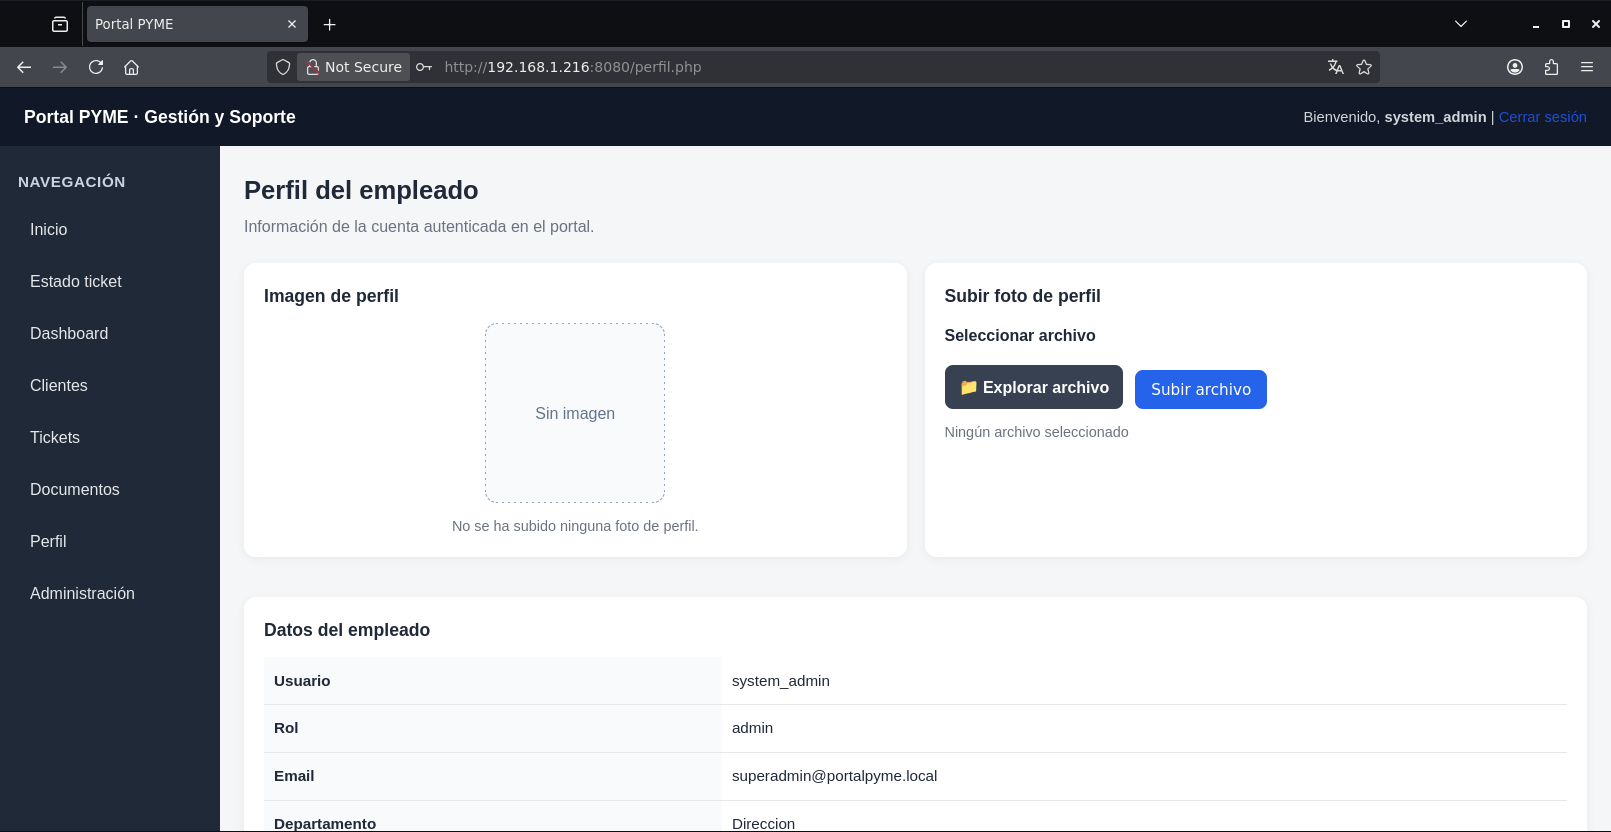
\includegraphics[width=0.85\textwidth]{Imagenes/portal_interno.png}

    \vspace{0.2cm}
    \captionazul{Acceso al panel interno del Portal PYME tras explotar el formulario de autenticación.}
    \label{fig:portal_interno}
\end{figure}

Una vez dentro del portal, se analizó el módulo de tickets, especialmente el endpoint público encargado de consultar el estado de una incidencia mediante el parámetro \texttt{codigo}. Partiendo de un identificador válido, como \texttt{TCK-2026-001}, se comprobó que dicho parámetro era incorporado directamente en una consulta SQL sin una validación adecuada. La introducción de caracteres de control y consultas \texttt{UNION SELECT} permitió confirmar la vulnerabilidad, determinar el número de columnas de la consulta y extraer información de la base de datos.

Mediante esta técnica se recuperó información sensible de la tabla \texttt{empleados}, incluyendo nombres de usuario, contraseñas y roles internos. Entre los datos obtenidos destacaba la cuenta \texttt{system\_admin}, asociada a privilegios administrativos dentro del portal. Esta evidencia confirma que la vulnerabilidad del módulo de tickets podía utilizarse tanto para exfiltrar información como para obtener credenciales válidas de la aplicación.

\begin{figure}[H]
    \centering
    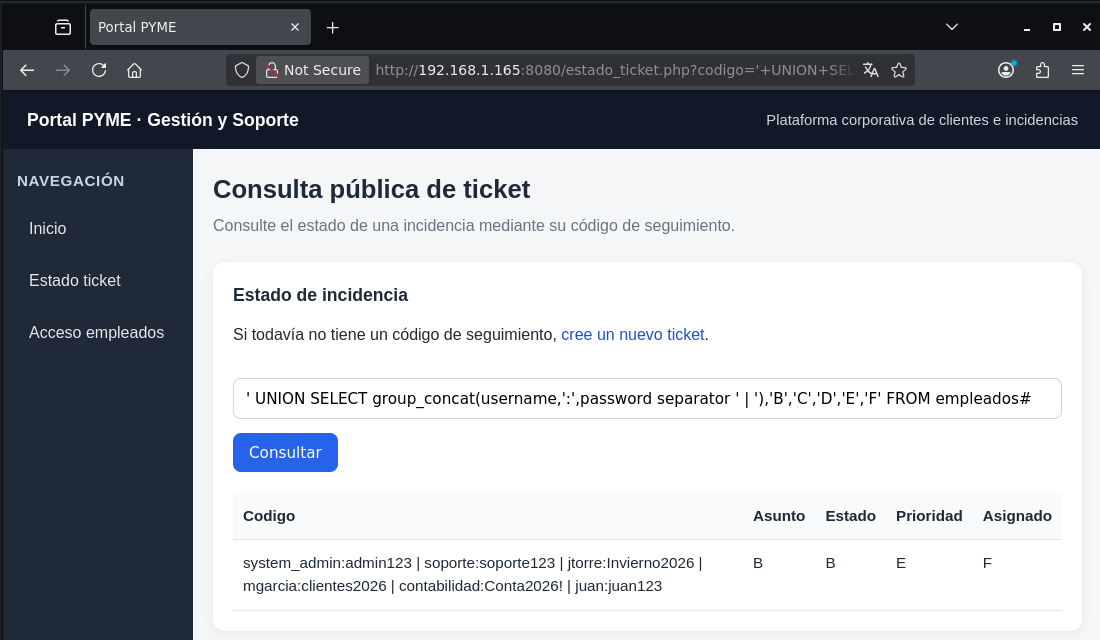
\includegraphics[width=0.85\textwidth]{Imagenes/leak-databas-tickets.png}

    \vspace{0.2cm}
    \captionazul{Extracción de credenciales desde la base de datos mediante SQL Injection en el módulo de tickets.}
    \label{fig:leak_database_tickets}
\end{figure}

Durante el análisis del módulo de tickets también se validaron dos debilidades adicionales. Por un lado, la creación de tickets permitía introducir contenido HTML y JavaScript que posteriormente era renderizado por la aplicación sin una codificación adecuada, dando lugar a un caso de Cross-Site Scripting almacenado. Por otro lado, los identificadores de ticket seguían un formato predecible, como \texttt{TCK-2026-001}, \texttt{TCK-2026-002} o \texttt{TCK-2026-003}. La modificación manual del parámetro \texttt{codigo} permitía consultar incidencias ajenas si no existía una comprobación de autorización asociada al usuario autenticado.

Estas dos vulnerabilidades no fueron necesarias para avanzar en la cadena principal de compromiso, pero permiten demostrar que el Portal PYME contiene varios vectores de explotación habituales en aplicaciones corporativas. En un entorno real, el XSS almacenado podría utilizarse para afectar a usuarios internos o administradores, mientras que el IDOR podría permitir la exposición de información perteneciente a otros usuarios.

\begin{figure}[H]
    \centering
    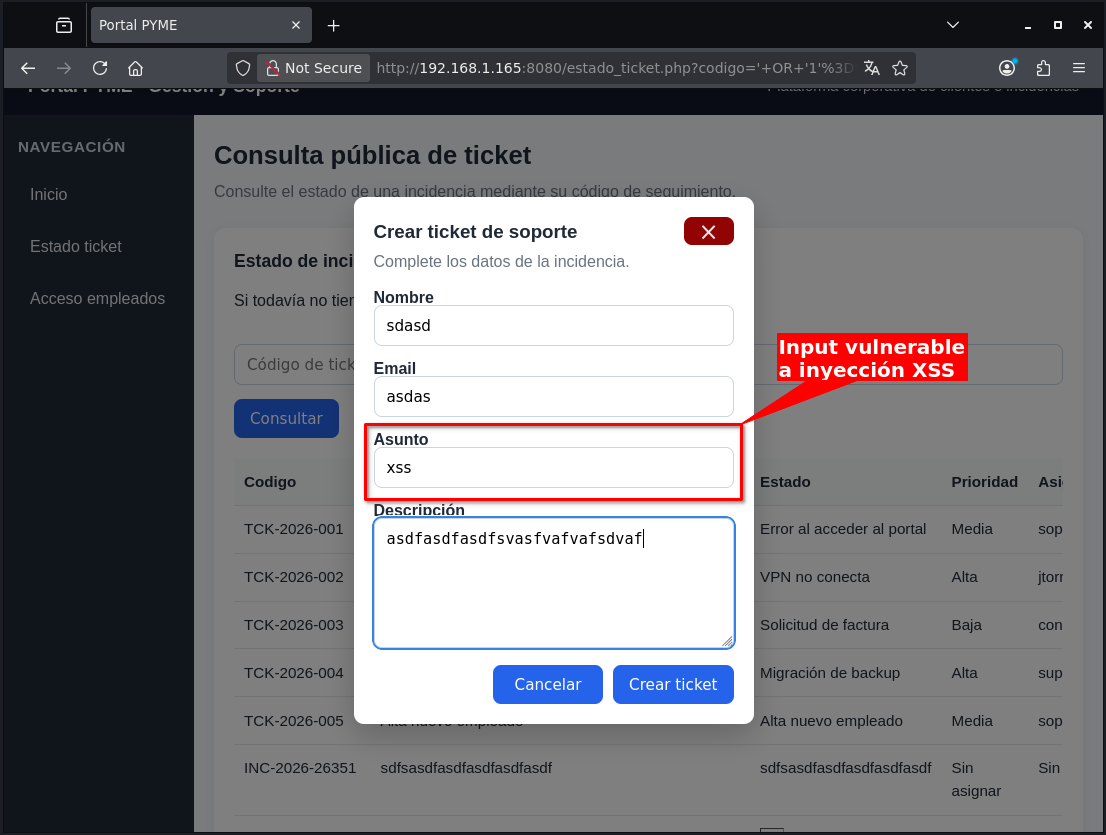
\includegraphics[width=0.85\textwidth]{Imagenes/xss-tickets.png}

    \vspace{0.2cm}
    \captionazul{Inserción de contenido controlado por el usuario en el módulo de tickets, representando un caso de XSS almacenado.}
    \label{fig:xss_tickets}
\end{figure}

\begin{figure}[H]
    \centering
    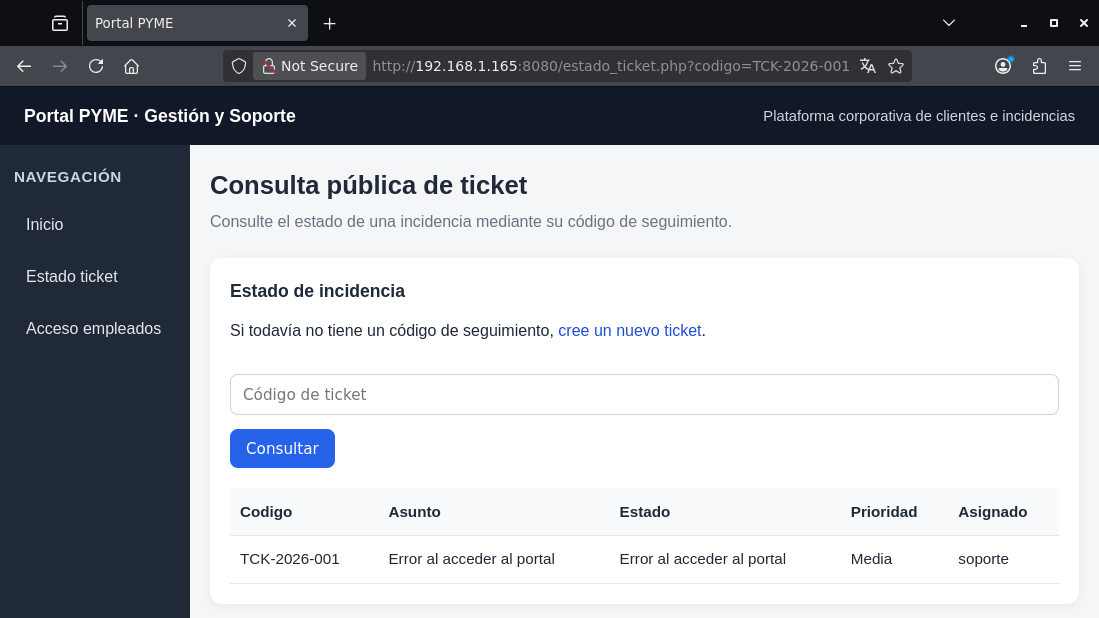
\includegraphics[width=0.85\textwidth]{Imagenes/IDOR-tickets.png}

    \vspace{0.2cm}
    \captionazul{Consulta de tickets mediante identificadores predecibles, representando un caso de IDOR.}
    \label{fig:idor_tickets}
\end{figure}

En conjunto, esta fase permitió validar que el portal web no actuaba como un simple punto de entrada aislado, sino como una superficie de ataque completa. La explotación del login permitió acceder al panel interno, la SQL Injection del módulo de tickets permitió recuperar credenciales y las vulnerabilidades XSS e IDOR demostraron la existencia de debilidades adicionales. Todo ello preparó el escenario para la siguiente fase de la cadena de ataque: la obtención de acceso inicial al servidor Ubuntu mediante la funcionalidad de subida de archivos.


% ---------------------------------------------------

\subsubsection{Acceso inicial al servidor Ubuntu}

Tras obtener acceso al panel interno, se identificó una funcionalidad de subida de imagen de perfil. Aunque la aplicación bloqueaba archivos PHP directos, el filtrado implementado resultó insuficiente, ya que aceptaba ficheros que simulaban ser imágenes pero conservaban una extensión interpretable por el servidor.

Este comportamiento permitió cargar un archivo híbrido con cabecera de imagen y código PHP. Al quedar almacenado en un directorio accesible desde el servidor web, el archivo pudo ser invocado desde el navegador, provocando ejecución remota de comandos en el servidor.

La ejecución del payload permitió obtener una reverse shell desde el servidor Ubuntu hacia la máquina atacante. El contexto inicial de ejecución correspondía al usuario del servicio web, \texttt{www-data}, lo que confirmó que el acceso inicial al sistema se había producido a través de la aplicación web.

\begin{figure}[H]
    \centering
    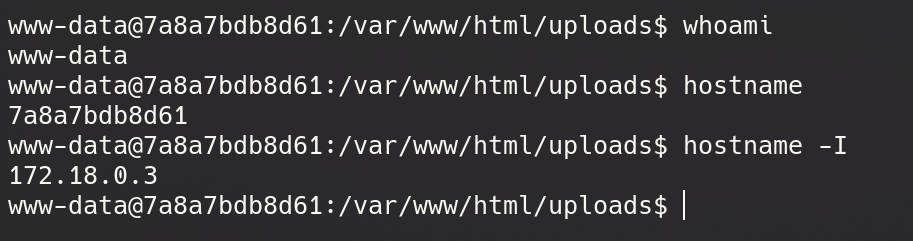
\includegraphics[width=0.85\textwidth]{Imagenes/www-data.png}

    \vspace{0.2cm}
    \captionazul{Obtención de una shell inicial con el usuario del servicio web.}
    \label{fig:www_data_shell}
\end{figure}

Esta fase representa el paso de una explotación puramente web a un compromiso inicial del servidor Ubuntu. A partir de este punto, el atacante deja de interactuar únicamente con la aplicación y obtiene capacidad de enumeración local sobre el sistema comprometido.

% ---------------------------------------------------

\subsubsection{Escalada de privilegios}

Una vez obtenida la shell inicial como \texttt{www-data}, se realizaron tareas de enumeración local sobre el servidor comprometido. Durante esta fase se identificó que el servicio web se ejecutaba dentro de un entorno contenerizado y que existían ficheros compartidos accesibles desde el contexto comprometido.

Entre los elementos encontrados se localizaron credenciales reutilizables asociadas al usuario \texttt{dev}. Estas credenciales permitieron abandonar el contexto limitado del usuario del servicio web y establecer una conexión SSH contra el servidor Ubuntu.

\begin{figure}[H]
    \centering
    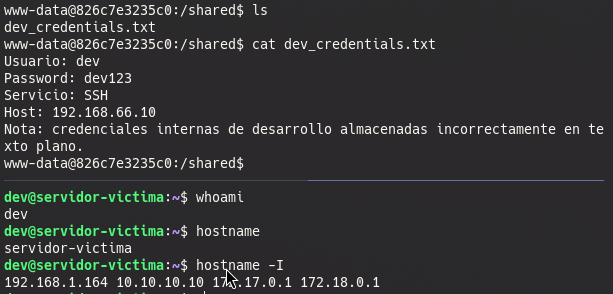
\includegraphics[width=1\textwidth]{Imagenes/escalada-privilegio-web.png}

    \vspace{0.2cm}
    \captionazul{Uso de credenciales recuperadas durante la post-explotación para acceder al servidor Ubuntu.}
    \label{fig:escalada_privilegio_web}
\end{figure}

La escalada permitió consolidar el acceso al servidor y disponer de una sesión más estable para continuar con las fases posteriores. Aunque el acceso inicial se obtuvo desde la aplicación web, esta fase permitió transformar dicho acceso en una posición más útil dentro del sistema operativo.

% ---------------------------------------------------

\subsubsection{Obtención de credenciales}

La obtención de credenciales constituye una fase clave dentro de la cadena de ataque, ya que permite conectar el compromiso del servidor web con el acceso a otros sistemas de la infraestructura.

Durante la explotación del portal se recuperaron credenciales almacenadas en la base de datos de la aplicación. Asimismo, durante la enumeración local del servidor Ubuntu se localizaron credenciales reutilizables asociadas a usuarios del laboratorio.

Estas credenciales permitieron avanzar desde un acceso limitado al servidor web hacia otros sistemas internos. En particular, la cuenta \texttt{dev} resultó relevante para acceder al servidor Ubuntu mediante SSH y posteriormente para validar el acceso a la estación de trabajo DEV01.

Esta fase demuestra el impacto que puede tener una gestión deficiente de credenciales dentro de un entorno corporativo. Una vulnerabilidad inicial en una aplicación web puede derivar en la exposición de usuarios y contraseñas que, si son reutilizadas en otros servicios, facilitan el movimiento lateral y amplían el alcance del compromiso.

% ---------------------------------------------------

\subsubsection{Movimiento lateral}

Tras consolidar el acceso al servidor Ubuntu, se comprobó que el sistema disponía de conectividad hacia una red interna adicional correspondiente al segmento \texttt{10.10.10.0/24}. Esta red no era accesible directamente desde la máquina atacante, por lo que fue necesario utilizar el servidor comprometido como punto de pivote.

Para ello se empleó Ligolo-ng, creando un túnel entre Kali Linux y el servidor Ubuntu comprometido. Una vez establecida la conexión y añadida la ruta correspondiente, fue posible enumerar la red interna desde la máquina atacante como si existiera conectividad directa.

\begin{figure}[H]
    \centering
    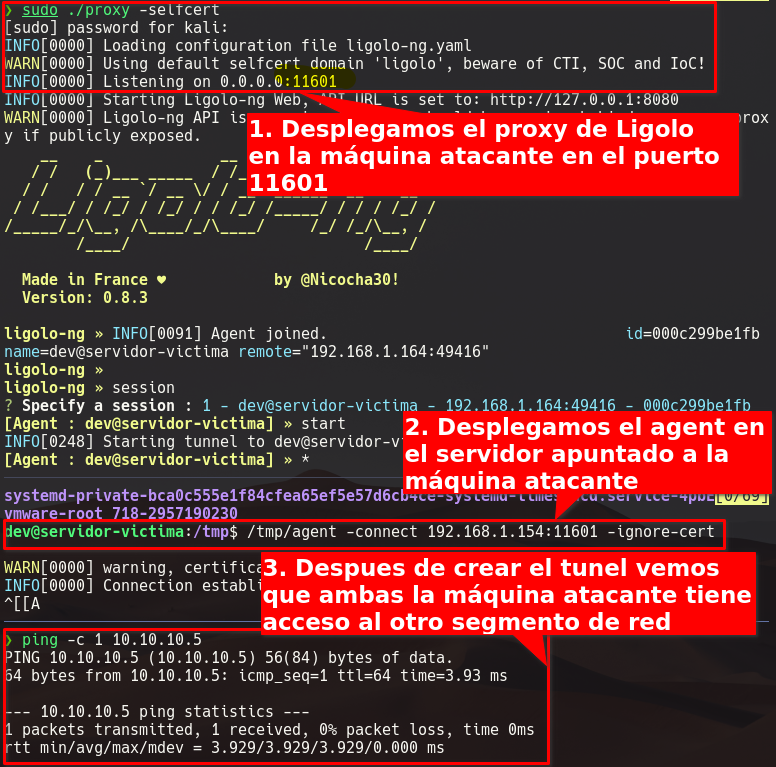
\includegraphics[width=0.85\textwidth]{Imagenes/ligolo.png}

    \vspace{0.2cm}
    \captionazul{Túnel de pivoting establecido hacia la red interna mediante Ligolo-ng.}
    \label{fig:ligolo_pivoting}
\end{figure}

La enumeración interna permitió identificar la estación \texttt{DEV01}, correspondiente a un equipo Windows 7 integrado en el entorno corporativo. El análisis de servicios reveló la presencia de SMB y RDP, lo que permitió validar el acceso remoto utilizando credenciales obtenidas en fases anteriores.

\begin{figure}[H]
    \centering
    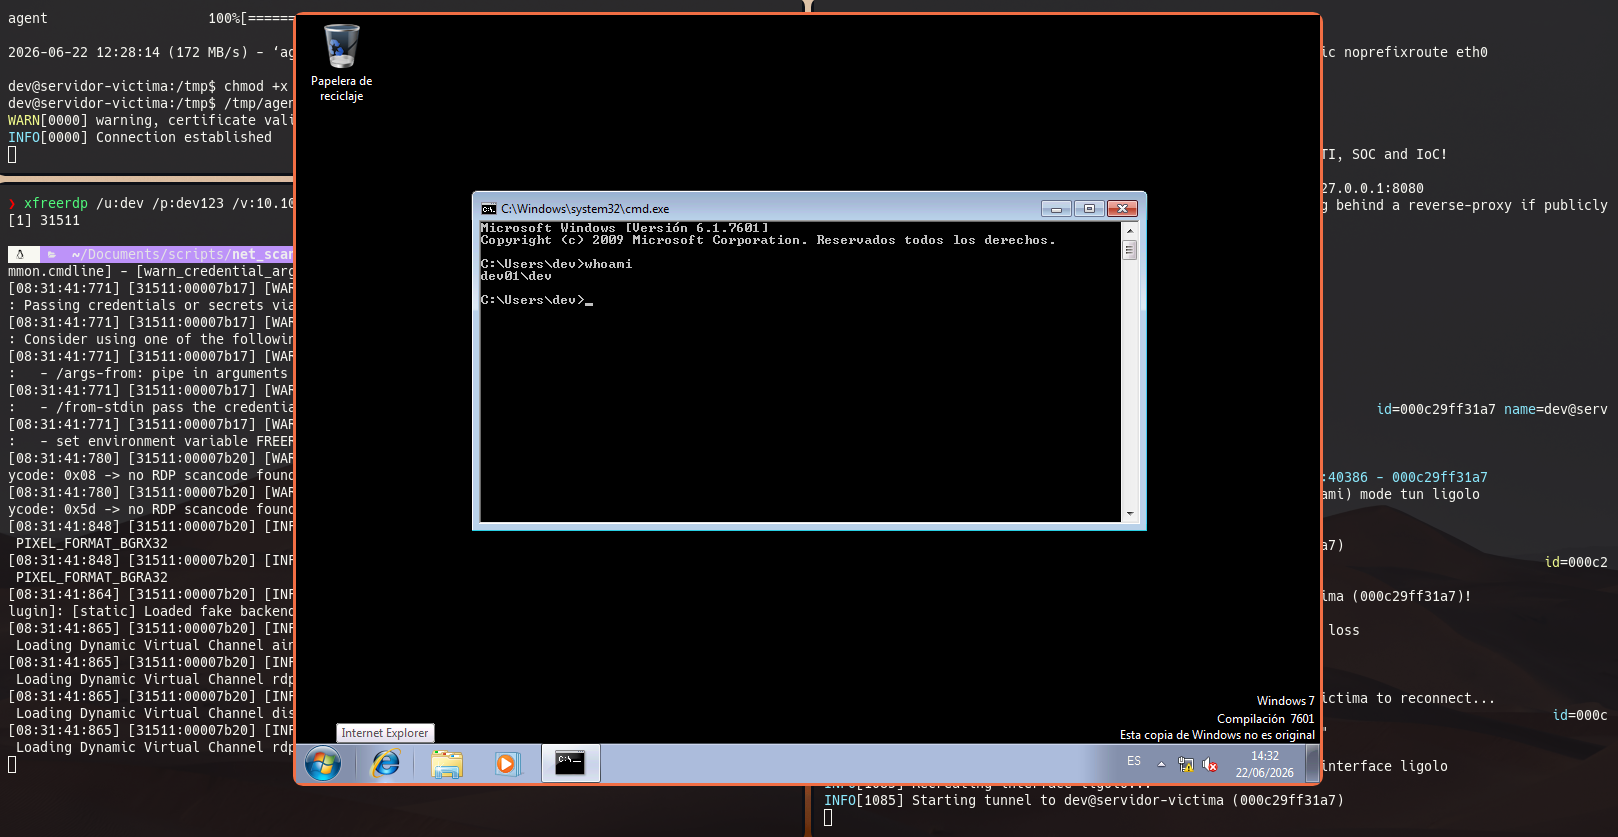
\includegraphics[width=0.85\textwidth]{Imagenes/RDP.png}

    \vspace{0.2cm}
    \captionazul{Acceso remoto a la estación DEV01 mediante RDP utilizando credenciales obtenidas previamente.}
    \label{fig:rdp_dev01}
\end{figure}

El compromiso de DEV01 representa la fase de movimiento lateral dentro de la infraestructura. A partir del servidor web inicialmente comprometido, el atacante consigue alcanzar un sistema interno que no era accesible de forma directa desde su posición inicial.

% ---------------------------------------------------

\subsubsection{Enumeración interna}

Una vez obtenida conectividad hacia la red interna, se procedió a enumerar los sistemas y servicios asociados a la infraestructura Active Directory. El objetivo de esta fase consistió en identificar el controlador de dominio, reconocer los servicios expuestos y recopilar información útil para el compromiso final.

El escaneo del sistema DC01 permitió identificar servicios característicos de un controlador de dominio Windows Server, como DNS, Kerberos, LDAP, SMB, Global Catalog, WinRM y Active Directory Web Services. La información obtenida permitió confirmar el nombre del equipo, el dominio \texttt{corp.local} y el rol del sistema dentro de la infraestructura.

\begin{figure}[H]
    \centering
    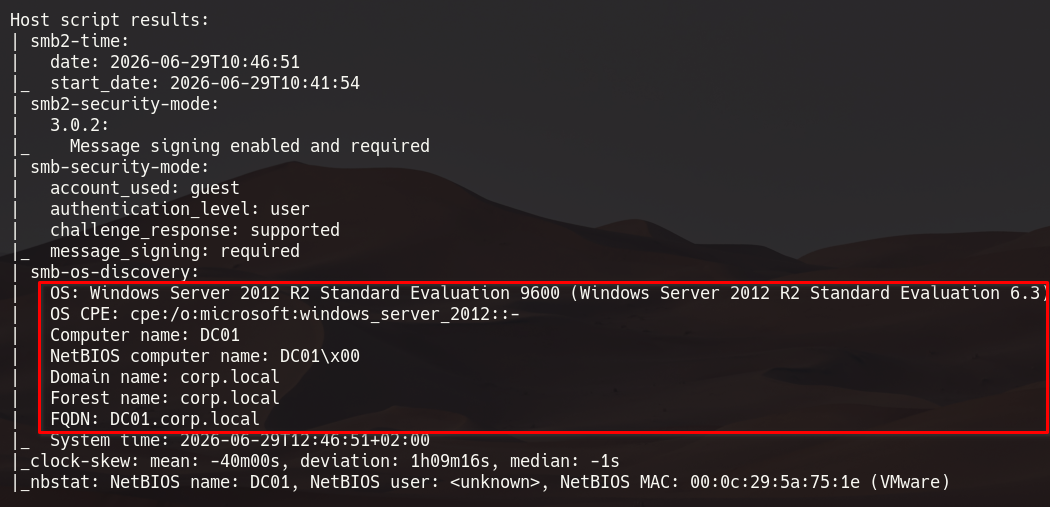
\includegraphics[width=0.85\textwidth]{Imagenes/scaneo-DC01-detalle.png}

    \vspace{0.2cm}
    \captionazul{Detalle de servicios expuestos por DC01, incluyendo servicios propios de Active Directory.}
    \label{fig:scaneo_dc01_detalle}
\end{figure}

Esta fase permitió validar que la segmentación de red y la infraestructura Active Directory se comportaban conforme al diseño planteado. El controlador de dominio no era accesible inicialmente desde la máquina atacante, pero sí podía ser alcanzado tras comprometer el servidor Ubuntu y establecer el túnel hacia la red interna.

% ---------------------------------------------------

\subsubsection{Compromiso final}

La fase final consistió en validar el acceso administrativo al controlador de dominio DC01. Para ello se realizaron pruebas controladas de autenticación contra los servicios SMB y WinRM utilizando credenciales y diccionarios reducidos adaptados al laboratorio.

El proceso permitió identificar credenciales válidas con privilegios administrativos sobre el dominio. Posteriormente, se verificó que dichas credenciales podían utilizarse mediante WinRM para establecer una sesión remota interactiva sobre DC01.

\begin{figure}[H]
    \centering
    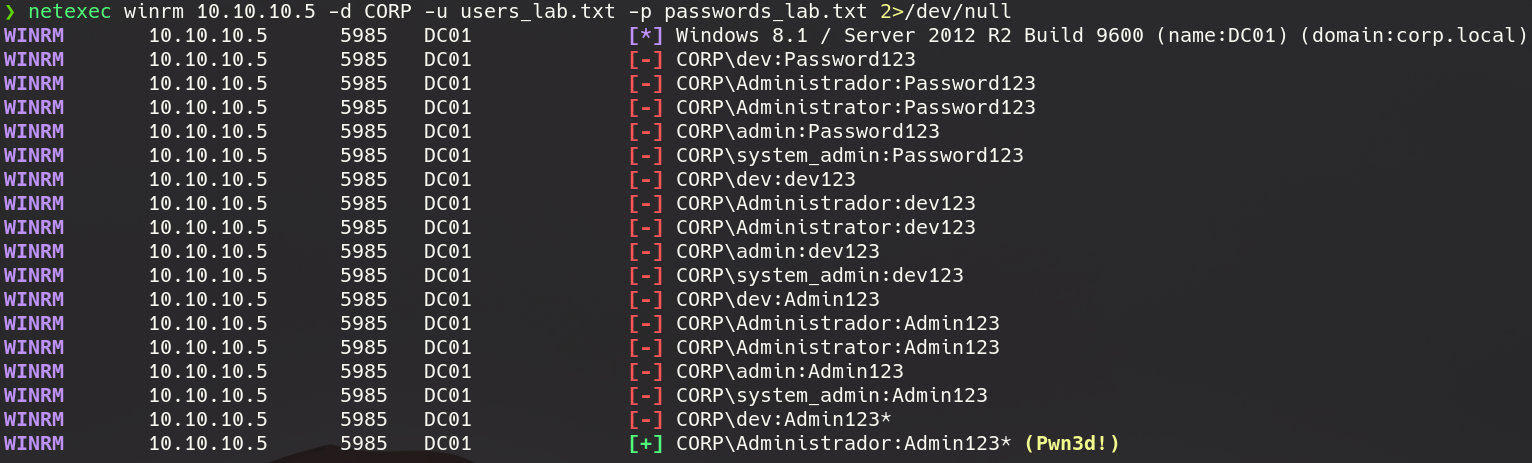
\includegraphics[width=\textwidth]{Imagenes/login-brute-force.png}

    \vspace{0.2cm}
    \captionazul{Validación de credenciales administrativas contra los servicios del controlador de dominio.}
    \label{fig:login_brute_force}
\end{figure}

\begin{figure}[H]
    \centering
    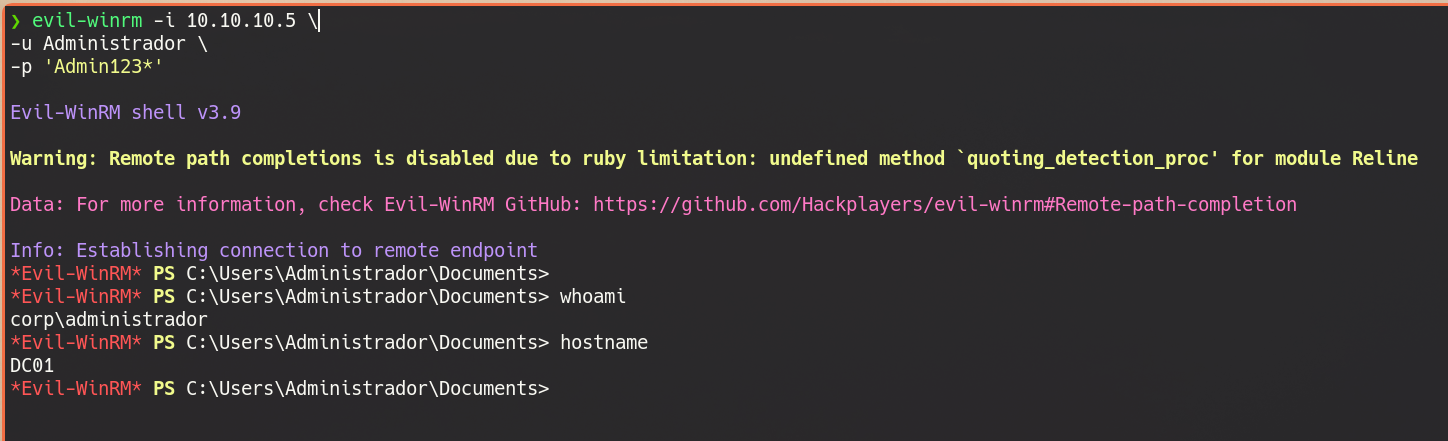
\includegraphics[width=1\textwidth]{Imagenes/evil-wnrm-DC01.png}

    \vspace{0.2cm}
    \captionazul{Acceso remoto al controlador de dominio DC01 mediante Evil-WinRM.}
    \label{fig:evil_winrm_dc01}
\end{figure}

La obtención de una consola PowerShell sobre DC01 confirmó el compromiso del controlador de dominio y, con ello, la culminación de la cadena de ataque planteada en el laboratorio. En este punto, el atacante alcanza el objetivo final del escenario: comprometer la infraestructura corporativa interna a partir de un acceso inicial obtenido mediante la aplicación web expuesta.

% ---------------------------------------------------

\subsection{Resumen de la cadena de ataque}

La explotación validada durante este capítulo puede resumirse como una cadena progresiva de compromiso. En primer lugar, se identifica el portal web expuesto y se explotan vulnerabilidades presentes en la aplicación. Posteriormente, se obtiene acceso inicial al servidor Ubuntu mediante una carga de archivos insegura y ejecución remota de comandos. A continuación, se escalan privilegios y se recuperan credenciales que permiten pivotar hacia la red interna.

Una vez alcanzada la red interna, el atacante compromete la estación DEV01 y enumera los servicios asociados a Active Directory. Finalmente, mediante credenciales válidas y acceso remoto por WinRM, se obtiene control sobre el controlador de dominio DC01.

\begin{center}
\begin{tikzpicture}[
    node distance=0.6cm,
    fase/.style={
        rectangle,
        rounded corners,
        draw=blueColor,
        fill=blue!8,
        text width=7cm,
        align=center,
        minimum height=0.9cm,
        font=\small
    },
    sistema/.style={
        rectangle,
        rounded corners,
        draw=red!70,
        fill=red!8,
        text width=7cm,
        align=center,
        minimum height=0.9cm,
        font=\small
    },
    final/.style={
        rectangle,
        rounded corners,
        draw=green!70,
        fill=green!8,
        text width=7cm,
        align=center,
        minimum height=0.9cm,
        font=\small
    },
    flecha/.style={
        -{Latex[length=2.5mm]},
        thick
    }
]

\node[fase] (recon) {1. Reconocimiento\\Enumeración de servicios expuestos};
\node[fase, below=of recon] (web) {2. Explotación web\\Portal PYME vulnerable};
\node[sistema, below=of web] (ubuntu) {3. Acceso inicial\\Servidor Ubuntu};
\node[fase, below=of ubuntu] (priv) {4. Escalada de privilegios\\Compromiso del servidor};
\node[fase, below=of priv] (creds) {5. Obtención de credenciales\\Usuarios y servicios internos};
\node[sistema, below=of creds] (lateral) {6. Movimiento lateral\\DEV01};
\node[sistema, below=of lateral] (ad) {7. Enumeración interna\\Active Directory / DC01};
\node[final, below=of ad] (dominio) {8. Compromiso final\\Infraestructura corporativa};

\draw[flecha] (recon) -- (web);
\draw[flecha] (web) -- (ubuntu);
\draw[flecha] (ubuntu) -- (priv);
\draw[flecha] (priv) -- (creds);
\draw[flecha] (creds) -- (lateral);
\draw[flecha] (lateral) -- (ad);
\draw[flecha] (ad) -- (dominio);

\end{tikzpicture}
\end{center}

Esta secuencia demuestra cómo vulnerabilidades inicialmente asociadas a una aplicación web pueden derivar en el compromiso de sistemas internos. El laboratorio permite reproducir de forma controlada una intrusión completa, combinando explotación web, exposición de credenciales, pivoting, movimiento lateral y abuso de servicios de administración remota.
